\section{Возможные пути и методы решения проблем}

\subsection{Методы сбора трафика}

3.1.1  NetFlow --- сетевой протокол, предназначенный для учёта сетевого трафика, разработанный компанией Cisco Systems. Является фактическим промышленным стандартом и поддерживается не только оборудованием Cisco, но и многими другими устройствами (в частности, Juniper, ZTE и Enterasys). Также существуют свободные реализации для UNIX-подобных систем.\par

Netflow предоставляет возможность анализа сетевого трафика на уровне сеансов, делая запись о каждой транзакции TCP/IP. Информация не столь подробна, как предоставляемая tcpdump'ом, но представляет довольно подробную статистику.\par 

Netflow имеет три основых компонента:
\begin{itemize}
	\item сенсор;
	\item коллектор;
	\item система обработки и представления данных.
\end{itemize}

\begin{figure}[h!]
    \centering
    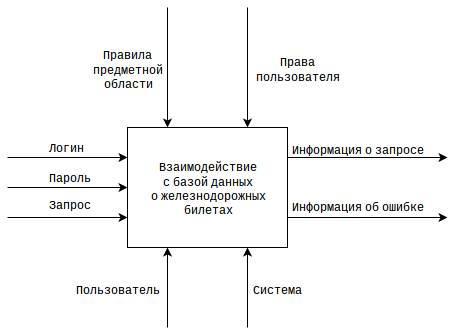
\includegraphics[width=0.65\textwidth]{1}
    \caption{Структура протокола Netflow}
    \label{img:1}
\end{figure} 

Сенсор --- демон, который слушает сеть и фиксирует данные сеанса. Коллектор должен иметь возможность подключиться к хабу, <<зеркалированному>> порту коммутатора или любому другому устройству, для просмотра сетевого трафика. Если вы используете систему пакетной фильтрации на базе BSD или Linux, то это превосходное место для коллектора Netflow, так как весь трафик будет проходить через эту точку. Сенсор будет собирать информацию о сеансах и сбрасывать ее в коллектор.\par 

Коллектор --- второй демон, который слушает на UDP порту, указанному вами и осуществляет сбор информации от сенсора. Полученные данные он сбрасывает в файл для дальнейшей обработки. Различные коллекторы сохраняют данные в различных форматах.\par 

Система обработки читает эти файлы и генерирует отчеты в форме, более удобной для человека. Эта система должна быть совместима с форматом данных, предоставляемых коллектором. \par 

Обычно коллектор и анализатор являются частями одного программного комплекса, работающего на сервере. Разновидностей ПО коллектор/анализатор множество, платные и бесплатные, под Windows и Unix-системы.\par 

Коллектор и стоящий за ним анализатор являются <<пассивными>> элементами системы. Сенсор шлет на коллектор отчеты о трафике, коллектор принимает, анализатор анализирует, и заполняет свою базу данных на сервере. По сути, при поднятом сервере, не нужно вручную подключать устройства, подпадающие под мониторинг, на сервере. Пока сенсор шлет отчеты, коллектор их принимает, анализатор регистрирует. Если сенсор выключен, он <<исчезает>> из текущей <<онлайн>> статистики.\par

Ввиду того, что этот протокол в большей степени предназначен для сбора статистики по трафику, сложно технически реализуем, а также не позволит производить глубокий анализ трафика в режиме реального времени, этот протокол решено не использовать.\par

3.1.2  tcpdump (от TCP и англ. dump --- свалка, сбрасывать) --- утилита UNIX (есть клон для Windows), позволяющая перехватывать и анализировать сетевой трафик, проходящий через компьютер, на котором запущена данная программа.\par 

Для выполнения программы требуется наличие прав суперпользователя и прямой доступ к устройству (так, например, запуск из Jail во FreeBSD невозможен).\par 

Основные назначения tcpdump в основном используется для отладки сетевых приложений и сети и сетевой конфигурации в целом.\par  

Программа состоит из двух основных частей: части захвата пакетов (обращение к библиотеке, libpcap (Unix) или pcap (Windows)) и части отображения захваченных пакетов (которая на уровне исходного кода является модульной и для поддержки нового протокола достаточно добавить новый модуль).\par 

Часть захвата пакетов (при запуске) передаёт <<выражение выбора пакетов>> (идущее после всех параметров командной строки) напрямую библиотеке захвата пакетов, которая проверяет выражение на синтаксис, компилирует его (во внутренний формат данных), а затем копирует во внутренний буфер программы сетевые пакеты, проходящие через выбранный интерфейс и удовлетворяющие условиям в выражении.\par 

Часть отображения пакетов выбирает захваченные пакеты по одному из буфера, заполняемого библиотекой, и выводит их (в воспринимаемом человеком виде) на стандартный вывод построчно, в соответствии с заданным (в командной строке) уровнем детальности.\par 

Если задан подробный вывод пакетов, программа проверяет для каждого сетевого пакета, имеется ли у неё модуль расшифровки данных, и, в случае наличия, соответствующей подпрограммой извлекает (и отображает) тип пакета в протоколе или передаваемые в пакете параметры.\par 

Если программа tcpdump вызвана для прослушивания некоторого интерфейса, она переводит его в <<promiscuous mode>> --- <<неразборчивый режим>>. В этом режиме интерфейс ловит вообще все пакеты, которые до него добрались, а не только пакеты адресованные непосредственно ему. Таким образом, если сеть собрана не на коммураторах (switch), а на репитерах (hub), то tcpdump позволит перехватить трафик между посторонними машинами, т.е. подслушать разговор двух сторонних машин. Сказанное не означает, что перехват трафика невозможен в сети собранной на коммутаторах. Впрочем, интерфейс можно и не переводить в promiscous mode, если передать программе аргумент -p.\par 

Ввиду недостаточной скорости работы и невозможности глубокого анализа трафика в реальном времени, решено не использовать эту утилиту.\par 

3.1.3  NetLimiter --- коммерческое программное обеспечение для семейства ОС Windows NT, решающая проблему контроля сетевого трафика. NetLimiter после установки и запуска следит за деятельностью каждого приложения, использующего доступ к Интернету, а также активно управляет трафиком, контролируя скорость потока данных. Вы можете самостоятельно настроить скорость загрузки и отправки информации для каждого отдельного приложения или соединения.\par 

Также NetLimiter ведет подробную статистику по всем соединениям, отображая ее в виде графиков или таблиц.\par 

С ее помощью можно легко контролировать весь трафик приложений и программ. Отслеживать доступ в интернет сторонних программ и возможность блокировки входящего/исходящего трафика. Например, можно заблокировать доступ программе для отключения автоматических обновлений или проверки ключей или лицензий.\par 

Ввиду того, что NetLimiter --- программа для коммерческого использования, а также того, что ОС Windows не вписывается в существующую сетевую инфраструктуру, данное программное решение решено не использовать.\\

